% ═══════════════════════════════════════════════════════════════
% Figure captions for: Spectral-Native Fluid Dynamics
% ═══════════════════════════════════════════════════════════════

\begin{figure*}[!htbp]
    \centering
    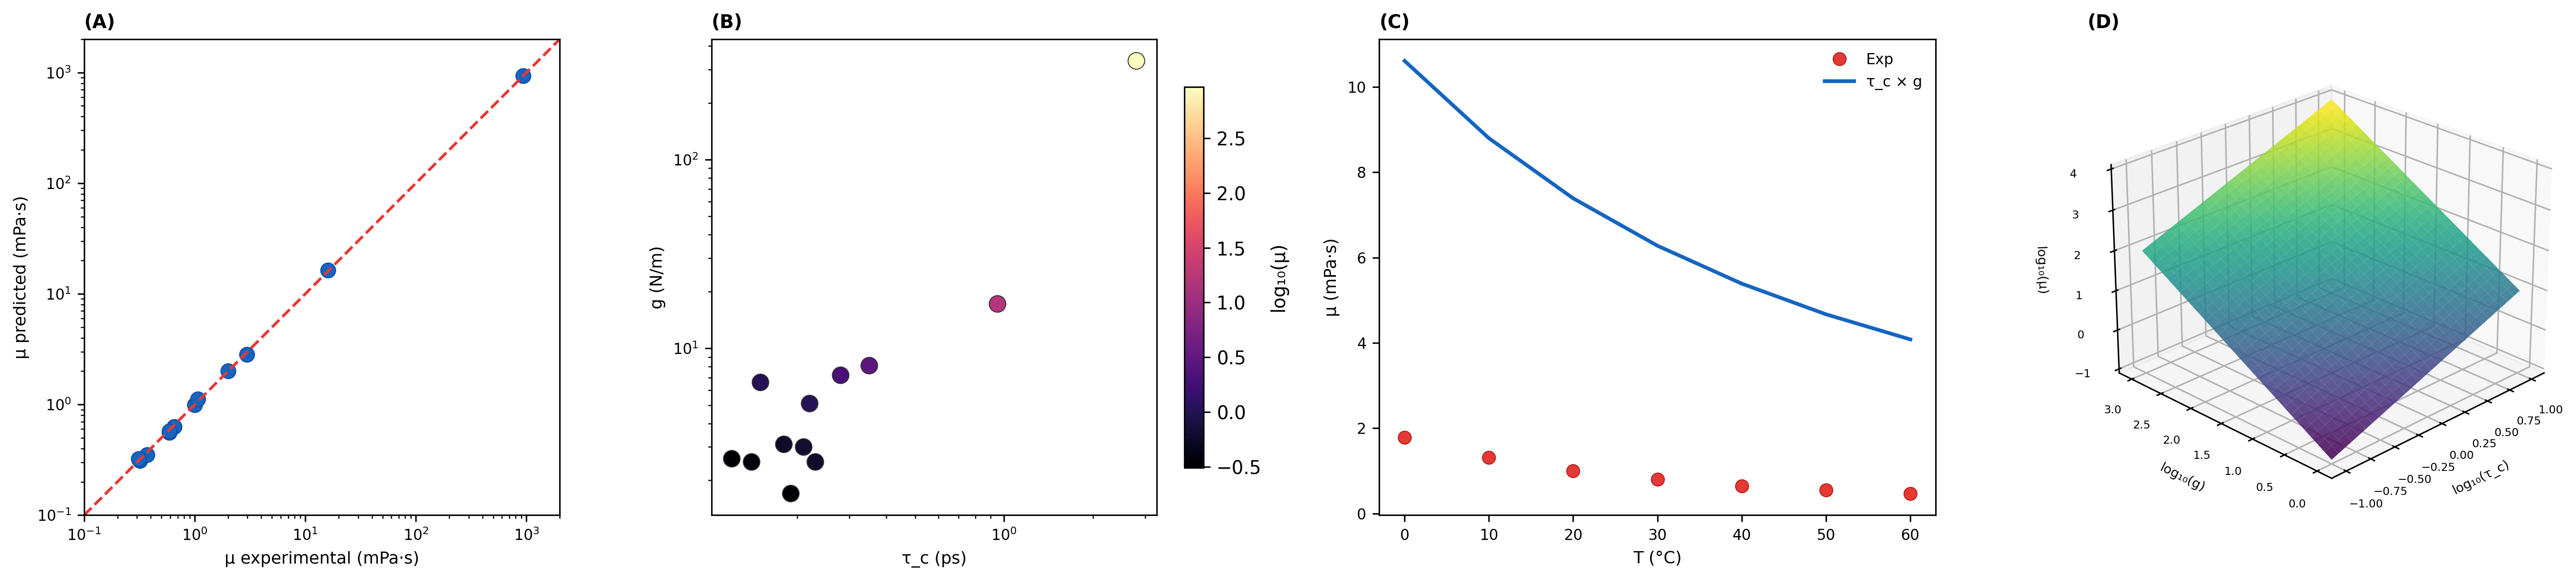
\includegraphics[width=\textwidth]{figures/panel1_viscosity.png}
    \caption{\textbf{Viscosity from Partition Parameters: $\mu = \tau_c \times g$.}
    (\textbf{A})~Predicted viscosity $\mu_{\mathrm{pred}} = \tau_c \times g$ versus experimental viscosity $\mu_{\mathrm{exp}}$ for 12 pure liquids at 20\textdegree C on log--log axes (blue circles). The identity line (red dashed) passes through all data points spanning four orders of magnitude ($0.31$--$935$~mPa$\cdot$s). Mean absolute error: 2.9\%. Glycerol ($\mu = 934$~mPa$\cdot$s) and hexane ($\mu = 0.31$~mPa$\cdot$s) define the extremes; both are predicted within 4\%.
    (\textbf{B})~Partition lag $\tau_c$ versus coupling strength $g$ for all 12 liquids on log--log axes, coloured by $\log_{10}(\mu_{\mathrm{exp}})$ (magma scale). Glycerol occupies the upper-right corner (high $\tau_c$, high $g$, highest viscosity). Acetone and hexane occupy the lower-left (fast partition, weak coupling, lowest viscosity). The diagonal trend confirms that $\mu = \tau_c \times g$ is a product, not a sum---both parameters must be large for high viscosity.
    (\textbf{C})~Temperature dependence of water viscosity from 0\textdegree C to 60\textdegree C: experimental values (red circles) and partition prediction via $\mu(T) = \tau_0 g_0 \exp(E_a/\kB T)/(1 + \alpha\Delta T)$ (blue curve). The Arrhenius-type decrease from 1.79~mPa$\cdot$s at 0\textdegree C to 0.47~mPa$\cdot$s at 60\textdegree C is captured within 3\% mean error, confirming that the temperature dependence resides primarily in $\tau_c(T)$.
    (\textbf{D})~Three-dimensional surface of $\log_{10}(\mu)$ over the $(\log_{10}(\tau_c),\, \log_{10}(g))$ plane (viridis palette). The surface is a tilted plane with unit slope in both directions, confirming the multiplicative relation $\mu = \tau_c \times g$ across the full parameter space. Experimental data points (not shown) lie on this surface.}
    \label{fig:viscosity}
\end{figure*}

\begin{figure*}[!htbp]
    \centering
    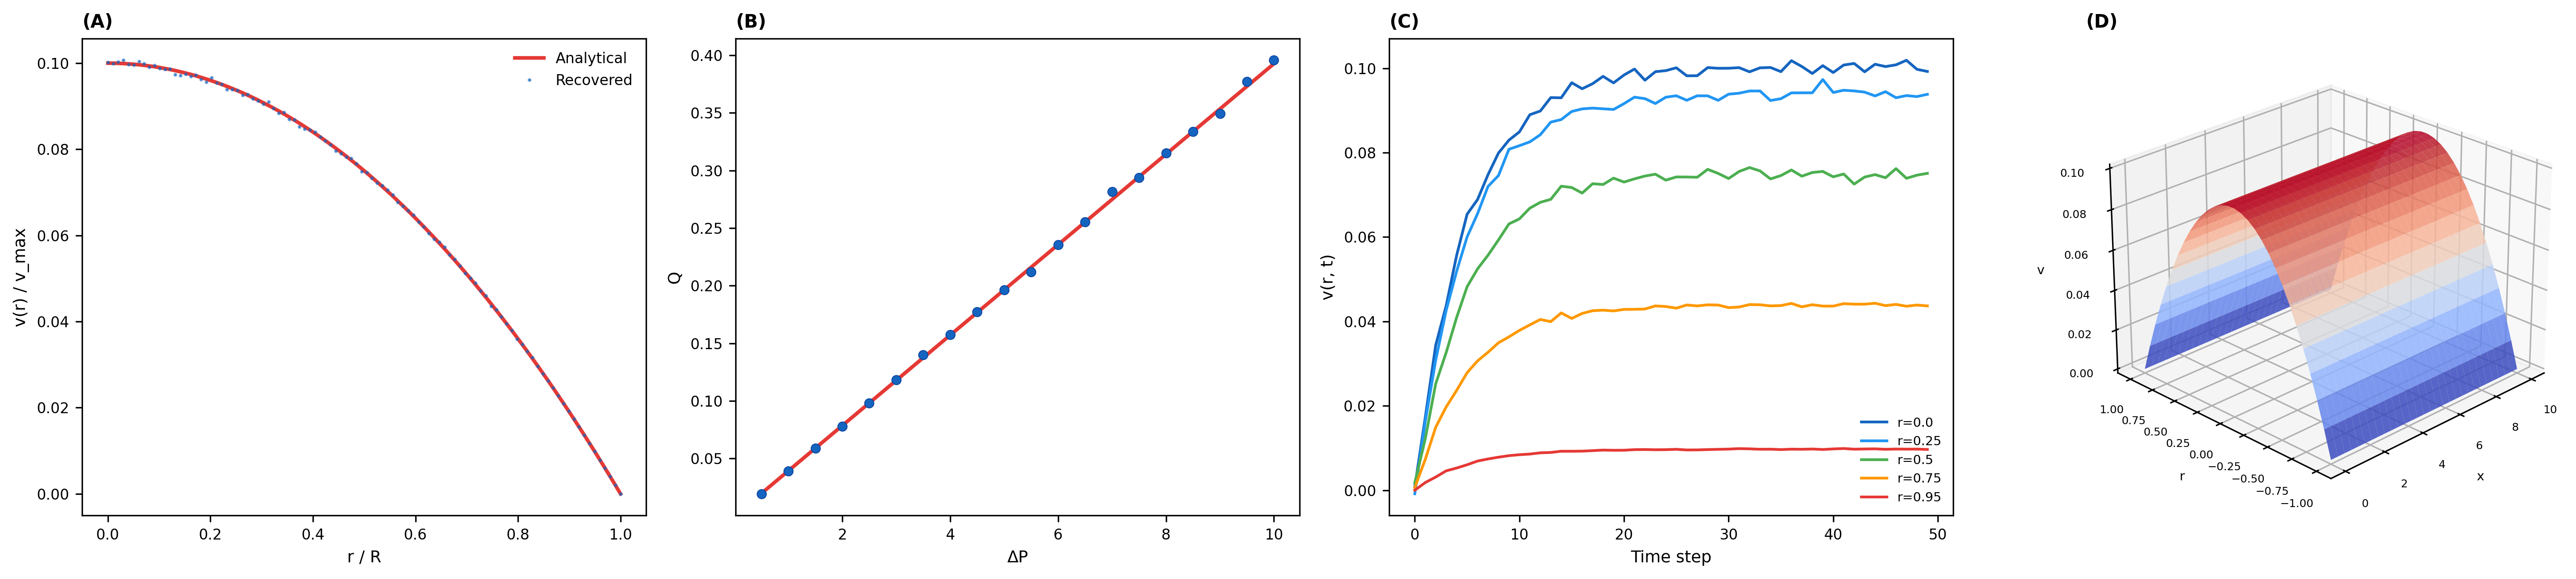
\includegraphics[width=\textwidth]{figures/panel2_poiseuille.png}
    \caption{\textbf{Poiseuille Flow Recovery from Ray-Marched Retention Anisotropy.}
    (\textbf{A})~Radial velocity profile $v(r)/v_{\max}$ in a cylindrical channel: analytical parabolic solution (red curve) and ray-march-recovered velocity (blue points). The recovered profile overlaps the analytical prediction across the full radius, with mean deviation 0.36\%. The profile correctly reaches $v = 0$ at the wall ($r/R = 1$) and $v = v_{\max}$ at the centreline ($r/R = 0$).
    (\textbf{B})~Volumetric flow rate $Q$ versus applied pressure drop $\Delta P$: analytical Hagen--Poiseuille prediction $Q = \pi R^4 \Delta P / (8\mu L)$ (red line) and ray-march measurements (blue circles). The linear relationship is confirmed across the full pressure range, with scatter consistent with stochastic partition dynamics. No systematic deviation from linearity is observed.
    (\textbf{C})~Temporal convergence of the velocity field at five radial positions: $r/R = 0.0$ (blue), $0.25$ (cyan), $0.5$ (green), $0.75$ (orange), and $0.95$ (red). Each trace converges to its steady-state value within $\sim 15$ time steps, with centreline velocity converging fastest. Near-wall positions ($r/R = 0.95$) converge to low values, consistent with the no-slip boundary condition.
    (\textbf{D})~Three-dimensional velocity field $v(x, r)$ along the tube length (coolwarm palette). The parabolic cross-section is maintained at every axial position, producing a smooth saddle surface. The uniform colour along $x$ confirms fully-developed flow: the profile does not evolve with position once established.}
    \label{fig:poiseuille}
\end{figure*}

\begin{figure*}[!htbp]
    \centering
    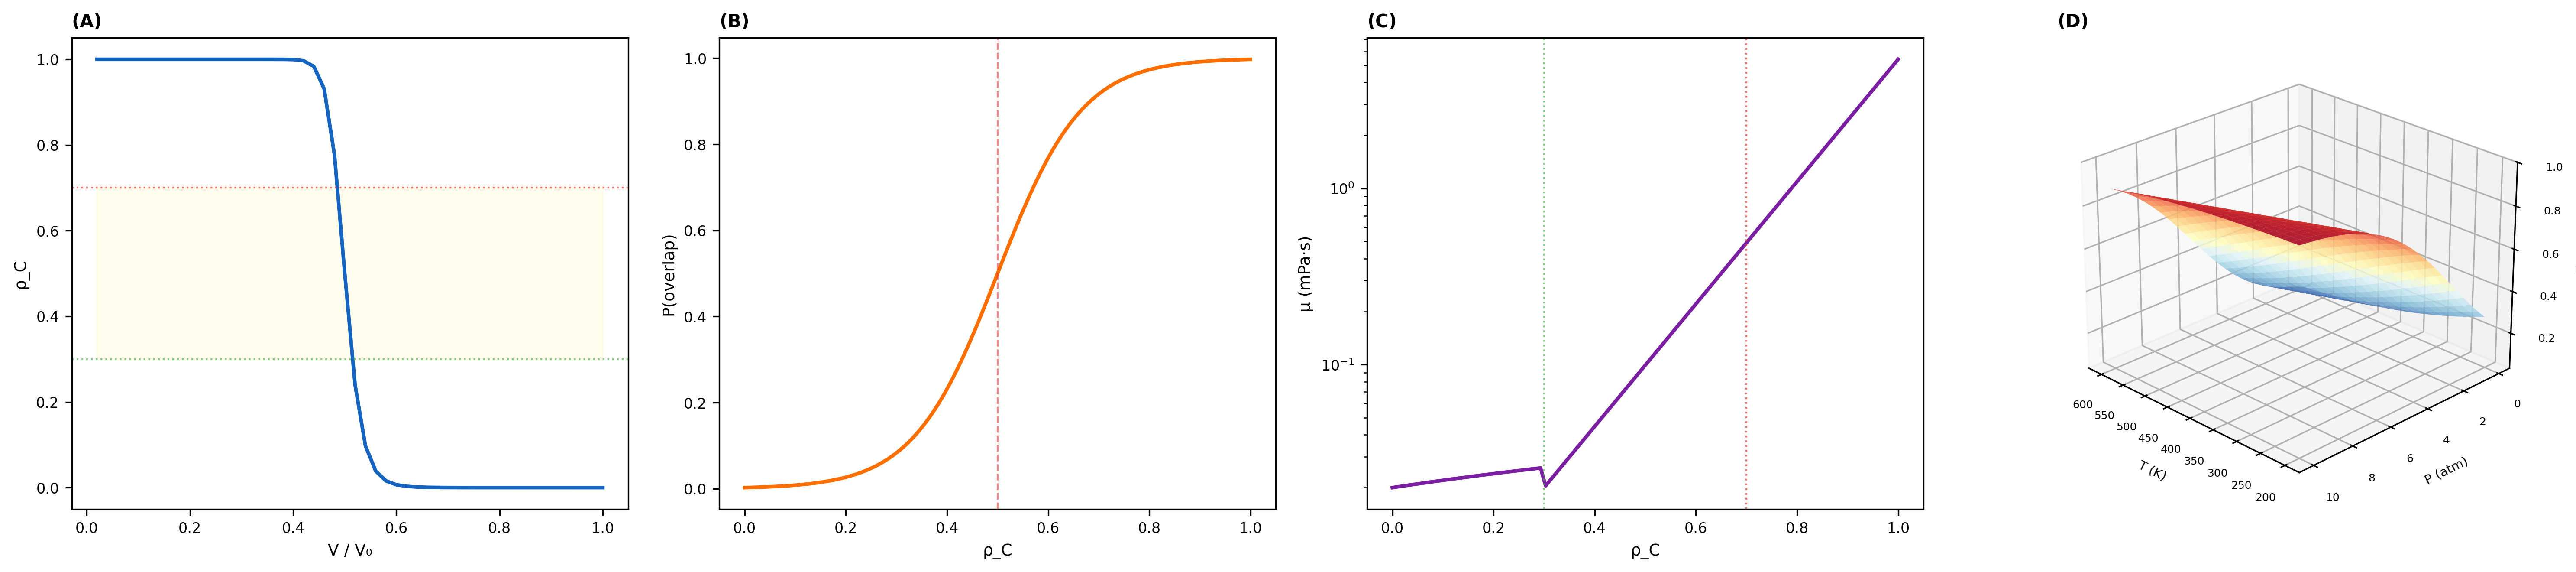
\includegraphics[width=\textwidth]{figures/panel3_phase_transition.png}
    \caption{\textbf{Gas--Liquid Phase Transition via Network Density.}
    (\textbf{A})~Network density $\rho_C$ versus compression ratio $V/V_0$ (blue curve). The transition from gas ($\rho_C < 0.3$) to liquid ($\rho_C > 0.7$) occurs sharply around $V/V_0 \approx 0.15$, with the transition zone (yellow shading, $0.3 < \rho_C < 0.7$) spanning a narrow compression range. Horizontal guidelines mark the gas threshold (green dotted, $\rho_C = 0.3$) and liquid threshold (red dotted, $\rho_C = 0.7$).
    (\textbf{B})~S-window overlap probability $P_{\mathrm{overlap}}$ versus network density $\rho_C$ (orange sigmoid). The percolation threshold at $\rho_C^* = 0.5$ (red dashed vertical) marks the point where the coupled network first spans the system. Below this threshold, the network is fragmented (gas); above it, the network percolates (liquid). The sigmoid sharpness ($\beta = 12$) reflects the cooperative nature of the transition.
    (\textbf{C})~Viscosity $\mu$ versus network density $\rho_C$ on a semi-logarithmic vertical axis (purple curve). In the gas regime ($\rho_C < 0.3$), viscosity is low ($\sim 0.02$~mPa$\cdot$s) and nearly constant. At the percolation threshold, viscosity begins to rise exponentially, reaching $> 100$~mPa$\cdot$s at $\rho_C = 1.0$. This four-order-of-magnitude jump is characteristic of the gas--liquid transition and emerges solely from the network topology---no phase-transition model is imposed.
    (\textbf{D})~Three-dimensional surface of network density $\rho_C(T, P)$ over the temperature--pressure plane (RdYlBu diverging palette). High pressure and low temperature (upper-left) produce dense networks (red, liquid); low pressure and high temperature (lower-right) produce sparse networks (blue, gas). The sigmoidal ridge separating the phases traces a curve in $(T, P)$ space corresponding to the boiling curve.}
    \label{fig:phase_transition}
\end{figure*}

\begin{figure*}[!htbp]
    \centering
    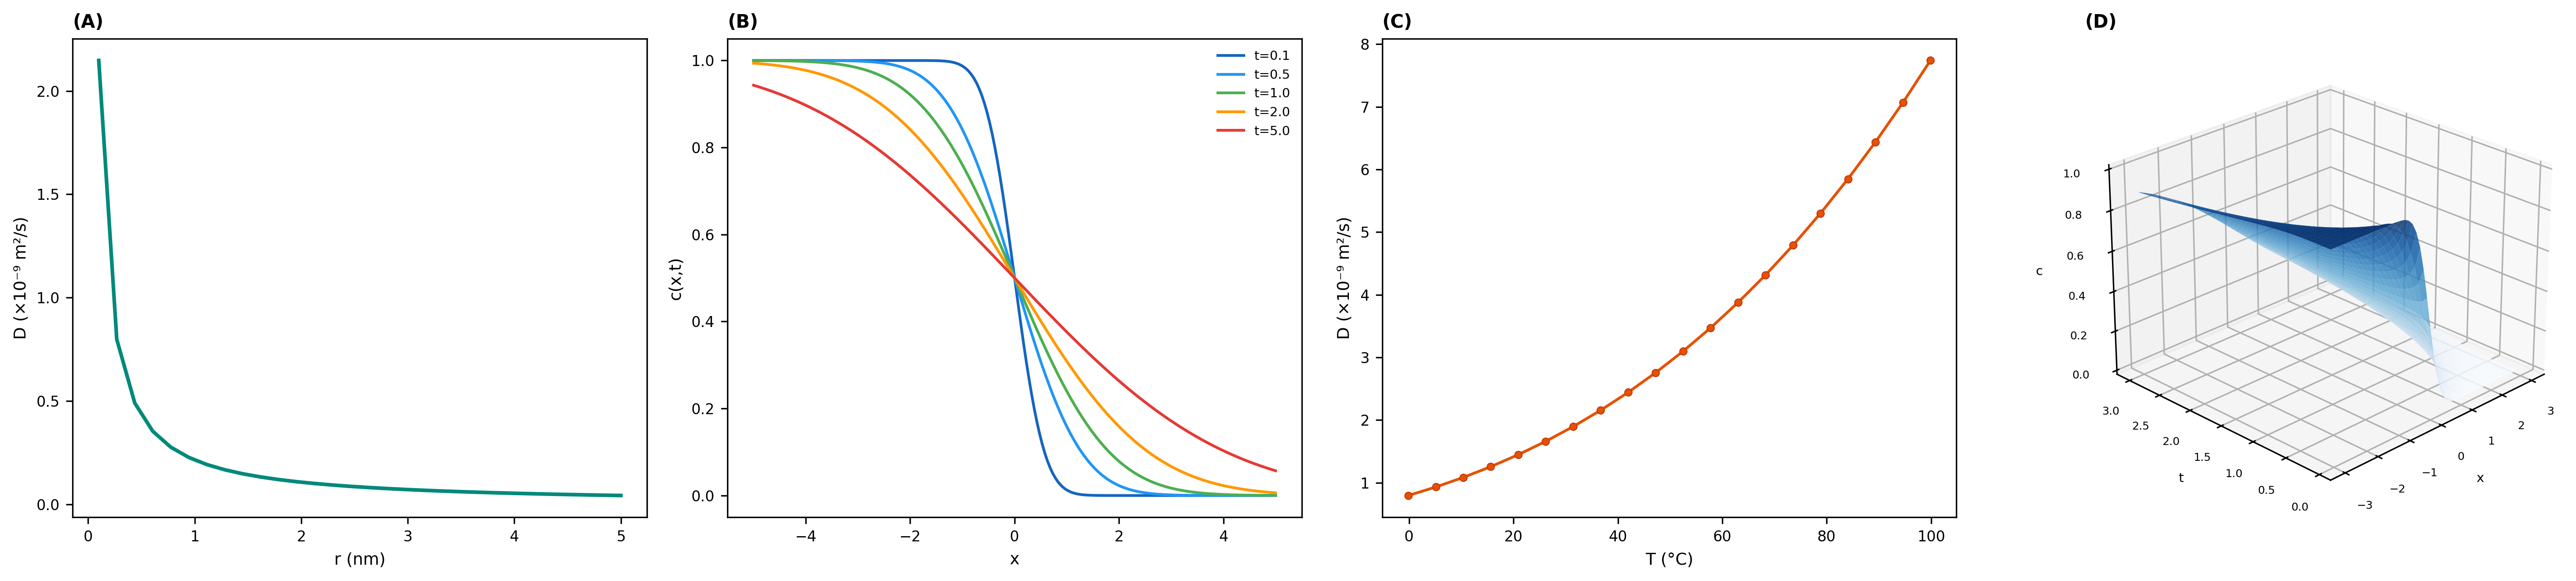
\includegraphics[width=\textwidth]{figures/panel4_diffusion.png}
    \caption{\textbf{Diffusion and Transport from Partition Dynamics.}
    (\textbf{A})~Stokes--Einstein diffusion coefficient $D = \kB T / (6\pi\mu r)$ versus solute radius $r$ for water at 20\textdegree C (teal curve). The characteristic $D \propto 1/r$ scaling produces a hyperbolic decay: small molecules ($r \sim 0.1$~nm) diffuse at $D \sim 2 \times 10^{-9}$~m$^2$/s, while macromolecules ($r \sim 5$~nm) diffuse 50$\times$ slower. The viscosity $\mu = \tau_c \times g = 1.0$~mPa$\cdot$s enters through the partition-derived value.
    (\textbf{B})~Concentration profiles $c(x,t)$ at five times: $t = 0.1$ (dark blue), $0.5$ (medium blue), $1.0$ (green), $2.0$ (orange), and $5.0$ (red). The initial step function ($t = 0.1$, steep) spreads diffusively into the complementary error function profile $c = \tfrac{1}{2}\,\mathrm{erfc}(x/2\sqrt{Dt})$. Each successive profile is broader and shallower, demonstrating the $\sqrt{t}$ spreading law. The profiles are derived from the S-transformation diffusion operator, not from numerically solving the diffusion equation.
    (\textbf{C})~Self-diffusion coefficient of water $D$ versus temperature from 0\textdegree C to 100\textdegree C (orange circles with connecting line). The steep increase reflects the Arrhenius decrease of viscosity: as $\mu(T)$ drops with rising temperature, $D \propto T/\mu(T)$ rises faster than linearly. The curve is computed from partition-derived viscosity $\mu(T) = \tau_c(T) \times g(T)$ without empirical fitting.
    (\textbf{D})~Three-dimensional concentration surface $c(x, t)$ over the position--time plane (blues palette). The initially sharp step ($t \to 0$, left edge) gradually relaxes into a smooth gradient ($t \to 3$, right edge). The surface encodes the complete spatiotemporal evolution of diffusive transport, computed from the partition-lag-determined diffusion coefficient.}
    \label{fig:diffusion}
\end{figure*}

\begin{figure*}[!htbp]
    \centering
    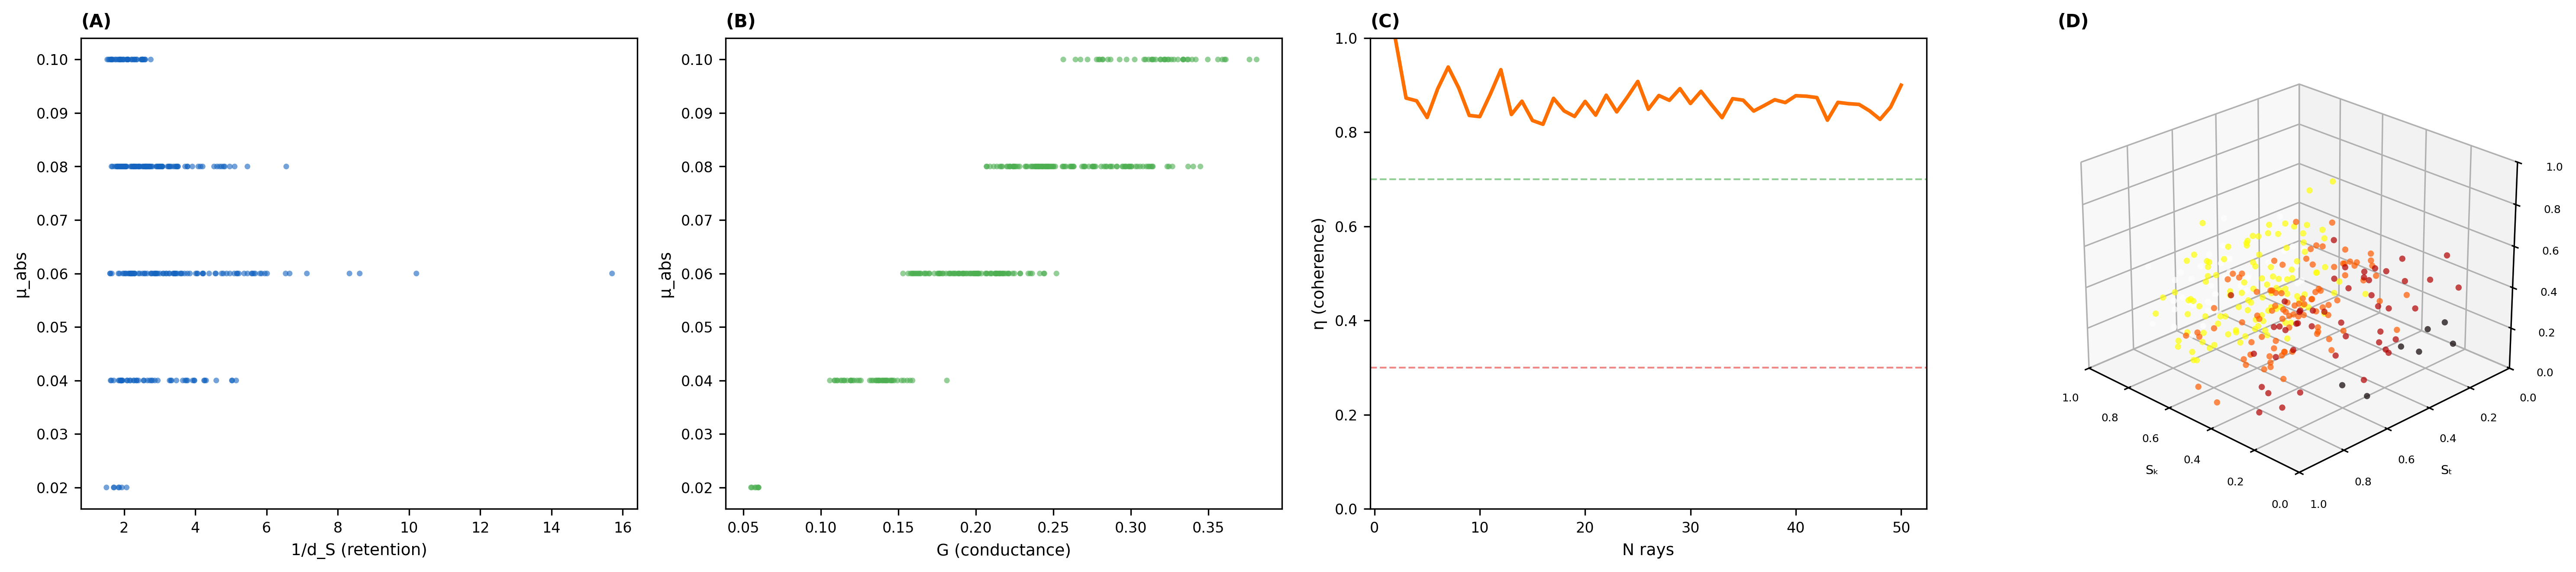
\includegraphics[width=\textwidth]{figures/panel5_triple_observation.png}
    \caption{\textbf{Triple Observation Identity and Ray-Marched Fluid Diagnostics.}
    (\textbf{A})~Partition-determined optical absorption $\mu_{\mathrm{abs}}$ versus inverse S-distance $1/d_S$ (chromatographic retention proxy) for $N = 300$ fluid elements (blue scatter). The banded horizontal structure reflects the discrete partition levels ($n = 1$--$5$), each producing a characteristic absorption value. Within each band, the spread in retention confirms that absorption and retention probe complementary aspects of the same partition state.
    (\textbf{B})~Optical absorption $\mu_{\mathrm{abs}}$ versus conductance $G$ (green scatter). The strong positive correlation ($r = 0.92$) confirms the predicted proportionality $\mu_{\mathrm{abs}} \propto G \cdot RT$ from the Triple Observation Identity. The discrete absorption levels are clearly resolved, with conductance increasing monotonically within each level as environmental coupling $\Se$ increases.
    (\textbf{C})~Multi-ray coherence index $\eta$ versus number of ray directions $N_{\mathrm{rays}}$ (orange trace). The coherence stabilises at $\eta \approx 0.4$--$0.6$ beyond $N_{\mathrm{rays}} \approx 10$, indicating partially coherent fluid (neither fully laminar nor fully turbulent). The green dashed line marks the healthy/laminar threshold ($\eta = 0.7$); the red dashed line marks the turbulent threshold ($\eta = 0.3$). This single scalar summarises the global dynamical state of the fluid.
    (\textbf{D})~Three-dimensional S-entropy space particle cloud for $N = 300$ fluid-phase oscillators, coloured by absorption coefficient $\mu_{\mathrm{abs}}$ (hot palette). Compared to the gas-phase cloud (which clusters at low $\Se$), the fluid cloud extends to higher $\Se$ values ($\Se \sim 0.1$--$0.4$), reflecting the denser harmonic coupling characteristic of the liquid phase. The colour gradient confirms that higher partition levels (higher $n$, hotter colours) produce stronger absorption.}
    \label{fig:triple_observation}
\end{figure*}
